\documentclass[a4paper,twoside,12pt]{article}
\usepackage{amsmath}
\usepackage{amsfonts}
\usepackage{amssymb}
\usepackage[utf8]{inputenc}
\usepackage[T1]{fontenc}
\usepackage{fancyhdr}
\usepackage{stmaryrd}
\usepackage{textcomp}
\usepackage[french]{babel}
\usepackage{variations}
\usepackage{psfrag,graphicx}
\usepackage{array}
\usepackage{verbatim}
\usepackage{psfrag}
\usepackage{bbm}
\usepackage{ifthen}
\usepackage[hmarginratio=3:4]{geometry}

\usepackage{listings}


\newlength{\myhoffset}
\newlength{\mytextwidth}
\newlength{\myvoffset}
\newlength{\mytextheight}
\setlength{\myhoffset}{-0.75cm}
\setlength{\mytextwidth}{1.5cm}
\setlength{\myvoffset}{-1.5cm}
\setlength{\mytextheight}{3cm}

\addtolength{\hoffset}{\myhoffset}
\addtolength{\textwidth}{\mytextwidth} 
\addtolength{\voffset}{\myvoffset}
\addtolength{\textheight}{\mytextheight} 

%\setlength{\oddsidemargin}{5mm}
%\setlength{\evensidemargin}{5mm}

%textpos : permet de placer des éléments par leur coordonnées absolues sur la page
% utilisé pour les entêtes et pied de pages

\usepackage[absolute]{textpos}
\setlength{\TPHorizModule}{1mm}
\setlength{\TPVertModule}{\TPHorizModule}
\textblockorigin{-\myhoffset}{-\myvoffset}

% appendix : permet d'écrire en couleur

\usepackage[usenames,dvipsnames,table]{xcolor}

% fancyhdr : permet de personnaliser les entêtes et pieds de page des documents

\usepackage{fancyhdr}

%% pdfpages : utilisé pour insérer la page de garde avant le document

\usepackage{pdfpages}

% caption : centre les légendes des figures

\usepackage[center]{caption}

% wrapfig : permet de créer des figures entourées de texte

\usepackage{wrapfig}

%placeins : permet d'obliger Latex à insérer les figures en attente avant de continuer

\usepackage{placeins}

% subcaption : permet de créer des figures avec plusieurs sous-figures

\usepackage{subcaption}

% appendix : permet de gérer les annexes

\usepackage[page]{appendix}

% multibib : permet d'organiser la bibliographie par catégories

\usepackage{multibib}

% layouts : affichage d'une longueur

\usepackage{layouts}

% tabularx : pour le tableau d'Antoine
\usepackage{color}
\usepackage{colortbl,arydshln}
\usepackage{tabularx}

% auto-pst-pdf : nécessaire pour insérer des formules latex dans un .eps, commenter la ligne suivante si vous n'avez pas ce package

\usepackage{auto-pst-pdf}
\usepackage{cutwin}
\usepackage{etex}

% eurosym : symbole euro

\usepackage{eurosym}

\usepackage{tocvsec2}

\setlength\parindent{0pt}

\linespread{1.1}


%%%% debut macro %%%%
\makeatletter
\def\hlinewd#1{%
\noalign{\ifnum0=`}\fi\hrule \@height #1 %
\futurelet\reserved@a\@xhline}
\makeatother
%%%% fin macro %%%%

\newcounter{partie}
\newcounter{sous-partie}

\renewcommand{\thesection}{\Roman{section}}

\newenvironment{partie}[1]
{
\section{#1}
}
{

}


\newcommand{\mymark}[1]{\markboth{\MakeUppercase{#1}}{\MakeUppercase{#1}}}

% Environnements représentants les parties du document

\newenvironment{intro}
{
\section*{Introduction}
\addcontentsline{toc}{section}{Introduction}
\mymark{Introduction}
}
{

}

\newenvironment{remerciements}
{
\section*{Remerciements}
\addcontentsline{toc}{section}{Remerciements}
\mymark{Remerciements}
}
{

}

\newenvironment{conclusion}
{
\section*{Conclusion}
\addcontentsline{toc}{section}{Conclusion}
\mymark{Conclusion}
}
{

}

\newenvironment{resume}
{
\section*{Résumé}
\addcontentsline{toc}{section}{Résumé}
\mymark{Résumé}
}
{

}


\newenvironment{sous-partie}[1]
{
\subsection{#1}
}
{

}

\newenvironment{sous-sous-partie}[1]
{
\subsubsection{#1}
}
{

}

\newenvironment{liste}
{
\vspace{0.2cm}
\begin{list}{$\bullet$\hspace{0.3cm}}{\leftmargin=1.4cm}
}
{
\end{list}
\vspace{0.2cm}
}

\newenvironment{oliste}
{
\vspace{0.2cm}
\begin{enumerate}
}
{
\end{enumerate}
\vspace{0.2cm}
}

\newcounter{numannexe}
\newenvironment{annexes}
{
\newpage
\setcounter{numannexe}{0}

\renewenvironment{partie}[1]
{
	\refstepcounter{subsection}
	\subsection*{\arabic{subsection}. ##1}
}
{
}

}
{

}

\newenvironment{annexe}[1]
{
\setcounter{subsection}{0}
\refstepcounter{numannexe}
\addcontentsline{toc}{subsection}{Annexe \arabic{numannexe} : #1}
\mymark{Annexe \arabic{numannexe} : #1}
\section*{Annexe \arabic{numannexe} : #1}
}
{
	\FloatBarrier
}

\newenvironment{sous-annexe}[1]
{
\begin{subappendices}
\subsection{#1}
}
{
\end{subappendices}
}


% Divers

% Permet de faire des cadres dans le document
\newcommand{\cadre}[1]{\renewcommand{\arraystretch}{0.4}\begin{array}{!{\vline}c!{\vline}}\hline\\#1\\\\\hline\end{array}}
\newcommand{\cadret}[1]{\renewcommand{\arraystretch}{0.4}\begin{tabular}{!{\vline}c!{\vline}}\hline\\#1\\\\\hline\end{tabular}}
\newcommand{\semicadre}[1]{\renewcommand{\arraystretch}{0.3}\begin{array}{c!{\vline}}#1\\\\\hline\end{array}}

% Commandes mathématiques

\newcommand{\equivalent}[2]{\!\!\renewcommand{\arraystretch}{1}\begin{array}[t]{c}\Huge\sim\\^{#1\rightarrow#2}\end{array}\!\!}
\newcommand{\tend}[2]{\!\renewcommand{\arraystretch}{1}\begin{array}[t]{c}-\!-\!\!\!\longrightarrow\\^{#1\rightarrow#2} \\ [-1.5ex]\end{array}\!}
\newcommand{\egal}[2]{\!\!\renewcommand{\arraystretch}{1}\begin{array}[t]{c}=\\^{#1\rightarrow#2}\end{array}\!\!}
\newcommand{\fin}{\vspace{0.2cm}\\}
\newcommand{\finq}{\vspace{0.5cm}\\}
\newcommand{\sh}{\mathrm{sh}\,}
\newcommand{\abs}[1]{\left\vert#1\right\vert }
\newcommand{\ch}{\mathrm{ch}\,}

\renewcommand{\o}[1]{\mathrm{o}\!\left(#1\right)}
\newcommand{\etoile}{\hspace*{1cm}$\star$\hspace*{0.5cm}}
\renewcommand{\th}{\mathrm{th}\,}
\renewcommand{\arcsin}{\mathrm{Arcsin}\,}
\renewcommand{\arccos}{\mathrm{Arccos}\,}
\newcommand{\argsh}{\mathrm{Argsh}\,}
\newcommand{\argch}{\mathrm{Argch}\,}
\newcommand{\argth}{\mathrm{Argth}\,}
\newcommand{\rg}{\mathrm{rg}\,}
\renewcommand{\arctan}{\mathrm{Arctan}\,}
\newcommand{\sq}{\hspace*{1.4cm}\stepcounter{sq}(\alph{sq})\hspace*{0.5cm}}
\newcommand{\rcl}{\begin{array}{rcl}}
\newcommand{\ea}{\end{array}}
\newcommand{\str}[1]{\renewcommand{\arraystretch}{#1}}
\renewcommand{\tfrac}[2]{\textstyle\frac{#1}{#2}}
\newcommand{\Cl}[1]{$C^{#1}$}
\newcommand{\mathCl}[1]{C^{#1}}
\renewcommand{\t}[1]{\tilde{#1}}
\renewcommand{\l}{\lambda}
\newcommand{\ds}{\displaystyle}
\newcommand{\R}{\mathbb{R}}
\newcommand{\C}{\mathbb{C}}
\newcommand{\Q}{\mathbb{Q}}
\newcommand{\Z}{\mathbb{Z}}
\newcommand{\N}{\mathbb{N}}
\newcommand{\Ker}{\mathrm{Ker}\,}
\newcommand{\Vect}{\mathrm{Vect}}
\renewcommand{\lvert}{\left\vert}
\renewcommand{\Im}{\mathrm{Im}\,}
\renewcommand{\rvert}{\right\vert}
\newcommand{\mnk}{\mathcal{M}_n(K)}
\newcommand{\mnc}{\mathcal{M}_n(C)}
\newcommand{\ppcm}{\mathrm{ppcm}}
\newcommand{\Tr}{\mathrm{Tr}\,}
\renewcommand{\t}[1]{^t\!#1}
\newcommand{\scal}[2]{\left\langle #1|#2\right\rangle}
\newcommand{\scalindice}[4]{\phantom{\langle}_{#3}\!\left\langle #1|#2\right\rangle_{#4}}
\newcommand{\p}[1]{\left( #1 \right)}
\newcommand{\crochet}[1]{\left[ #1 \right]}
\newcommand{\nr}[1]{\left\|\,#1\,\right\|}
\newcommand{\tab}{\hspace*{1cm}}

\newcommand{\esp}[1]{\mathbb{E}\!\crochet{#1}}
\newcommand{\espcond}[2]{\mathbb{E}_{#1}\!\crochet{#2}}

\renewcommand{\P}[1]{\mathbb{P}\!\p{#1}}
\newcommand{\Pcond}[2]{\mathbb{P}_{#1}\!\p{#2}}

\renewcommand{\binom}[2]{\left(\begin{array}{c}#1\\#2\end{array}\right)}

\newcommand{\car}[1]{\mathbf{1}_{#1}}

\newcommand{\matdd}[4]{\left({\begin{array}{cc} #1 & #2\\ #3 & #4 \ea}\right)\vspace{0.05cm}}

\newcommand{\supp}[1]{\text{supp}\left(#1\right)}

\renewcommand{\ge}{\geqslant}
\renewcommand{\le}{\leqslant}

\newcommand{\lebesgue}{\mathcal{L}}

\newcommand{\Drond}{\mathcal{D}}

\renewcommand{\Re}{\mathcal{R}e}
\newcommand{\obs}[1]{\hat{#1}}
\newcommand{\ket}[1]{\vert #1 \rangle}
\newcommand{\bra}[1]{\langle #1 \vert}
\newcommand{\braindice}[2]{\!\phantom{\langle}_{#2}\!\left\langle #1\right\vert}

\newcommand{\prodscal}[2]{\left\langle#1,#2\right\rangle}

\newcommand{\vect}[2]{\left(\str{1}\begin{array}{cc}#1 & #2 \ea\right)}
\newcommand{\vecttrans}[2]{\left(\str{1}\begin{array}{c}#1 \\ #2 \ea\right)}

\renewcommand{\v}[1]{\underline{#1}}

\newcommand{\Dp}[2]{\dfrac{\partial #1}{\partial #2}}
\newcommand{\grad}{\mathrm{grad}\,}
\newcommand{\vgrad}{\v{\mathrm{grad}}\,}




\def\br{\hfill\break\noindent}
\def\root{ \sqrt{ 1 - v^2/c^2}}
\def\p{\varphi}
\def\t{\theta}
\def\g{\gamma}
\def\a{\alpha}
\def\b{\beta}
\def\d{\delta}


\def\be{\begin{equation}}
\def\ee{\end{equation}}
\def\ba{\begin{eqnarray}}
\def\ea{\end{eqnarray}}
\def\ve{\overrightarrow}
\def\Vi{\ve{V_{\infty}}}
\def\Va{\ve{V_a}}
\def\v{\ve{v}}
\def\P{\ve{P}}
\def\Fa{\ve{F_a}}
\def\ex{\ve{e_x}}
\def\ey{\ve{e_y}}
\def\ez{\ve{e_z}}
\def\er{\ve{e_r}}
\def\et{\ve{e_{\t}}}
\def\ep{\ve{e_{\varphi}}}
\def\tp{\dot{\t}}
\def\tpp{\ddot{\t}}
\def\ro{\rho_0}
\def\M{\ve{M}}
\def\u{\ve{u}}
\def\n{\ve{n}}
\def\up{\ve{u_{\sslash}}}
\def\udeux{\ve{u_2}}
\def\l{\vec{l}}
\def\Da{\ve{D_a}}



\newcommand{\tablefigures}{

%\section*{Introduction}
%\addcontentsline{toc}{section}{Introduction}
%\mymark{Introduction}

\listoffigures

}


\pagestyle{fancy}

\setlength{\headheight}{2cm}

\renewcommand{\headrulewidth}{0.4pt}
\renewcommand{\footrulewidth}{0pt}

\fancyhead{}
\fancyfoot{}

\fancyhead[R]{
\includegraphics[height=1.5cm]{./images/Charte_graphique_polytechnique/logo_x_simple.png}}

\fancyfoot[RO,LE]{\thepage}
\fancyhead[L]{\leftmark}


\begin{document}

École polytechnique\hfill Mai 2012\\
Promotion 2010
\thispagestyle{empty}
\newlength{\margeimage}
\setlength{\margeimage}{1cm}
\vspace{\margeimage}
\begin{center}
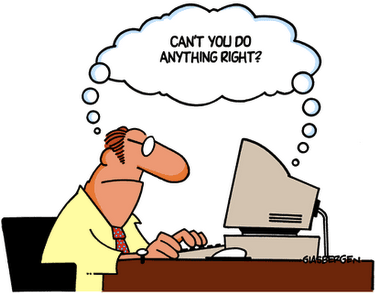
\includegraphics[width=8cm]{./images/blague.png}
\end{center}
\vspace{\margeimage}
\begin{center}
\begin{Large}
\bf
Projet de programmation INF431\vspace{0.3cm}\\
Rapport de fin de projet
\end{Large}
\end{center}
\vspace*{\fill}
\begin{flushright}
Thomas Brichard\\
Quentin Fiard
\end{flushright}

\clearpage


\settocdepth{subsection}

\tableofcontents

\vspace*{-0.4cm}

\begin{intro}
\begin{paragraph}{}
A l'ère du numérique et du développement massif d'internet, le plagiat de documents est devenu de plus en plus facile, et donc de plus en plus courant. Le type de documents plagiés est très variable, et peut aller d'un texte au code source d'un logiciel protégé, en passant par le code d'un site web.
\end{paragraph}
\vspace*{-0.3cm}
\begin{paragraph}{}
Des algorithmes ont été développés pour permettre de lutter contre ce fléau, notamment dans un cadre scolaire ou académique, et sont la plupart du temps fondés sur une comparaison d'une multitude de courts extraits des documents. Ce projet de programmation vise à mettre en pratique un de ces algorithmes, étudié dans un article de Schleimer, Wilkerson et Aiken\footnote{Saul Schleimer, Daniel S. Wilkerson, and Alex Aiken. Winnowing : local algorithme for document fingerprinting. In SIGMOD’03 : \textit{Proceedings of the 2003 ACM SIGMOD International Conference on Management of Data}, pages 76–85, 2003.}.
\end{paragraph}

\end{intro}

\clearpage

\begin{partie}{Organisation du travail de groupe}

Ce projet a été pour nous l'occasion de développer nos capacités de travail en équipe, et d'appréhender le processus de développement d'un programme informatique complexe. Nous détaillons dans cette partie la démarche que nous avons mise en place pour mener ce projet, et les outils qui nous ont permis un développement collaboratif du projet.

\begin{sous-partie}{Démarche mise en place}
\begin{paragraph}{}
Comme indiqué dans l'énoncé, nous avons cherché à décomposer au maximum le développement du projet en étapes élémentaires, à même d'être développées en parallèle.
\end{paragraph}
\begin{paragraph}{}
Nous avons dans un premier temps défini de façon précise l'architecture que nous allions mettre en place pour le projet (présentée dans la partie \ref{architecture}). Nous avons ensuite écrit les interfaces et les structures de données que nous allions utilisées par la suite (nous avons essayé au maximum d'écrire chaque partie indépendante du projet dans un package distinct, par soucis d'encapsulation). Nous avons ensuite développé chacun de notre côté différentes fonctionnalités du programme, avant de tester notre programme sur les exemples proposés.
\end{paragraph}
\end{sous-partie}

\begin{sous-partie}{Système de contrôle de versions}
\begin{figure}[htb]
\centering

\includegraphics[width=4cm]{./images/git.png}
\end{figure}

\begin{paragraph}{}
Pour nous permettre de développer en parallèle les fonctionnalités du programme, nous avons utilisé le système de contrôle de version git. Il nous a permis de fusionner les modifications de chacun au fur et à mesure, et nous à autoriser à tout moment à revenir à une version antérieur du code en cas de bugs de programmation. Il présente également l'avantage de pouvoir être utilisé hors ligne (contrairement à Dropbox par exemple, qui nécessite une connexion internet pour pouvoir conserver les différentes versions des fichiers).
\end{paragraph}

\begin{paragraph}{}
À cause du proxy de l'École, nous avons du mettre en place un répertoire de dépôt sur le réseau local de l'École, auquel git se connecte par ssh à l'aide d'un identifiant élève. La version finale du programme a également été mis en libre accès sur un dépôt Github\footnote{https://github.com/QuentinFiard/Plagiats/}.
\end{paragraph}

\end{sous-partie}

\end{partie}

\clearpage

\begin{partie}{Architecture du programme}
\label{architecture}

\begin{sous-partie}{Architecture globale du programme}
\begin{paragraph}{}
L'ensemble de l'exécution du programme est géré par la classe \texttt{Plagiats}. Elle prend en argument sur la ligne de commande les chemins d'accès aux fichiers ou aux dossiers dont les fichiers doivent être testés. On extrait ensuite de chaque fichier un ensemble d'empreintes représentatives du contenu du fichier. Pour chaque paire de fichiers, on cherche l'ensemble des empreintes communes, qui mettent en évidence des similarités entre les fichiers. Le programme affiche par la suite la liste des fichiers présentant des similarités, par ordre décroissant de similitude, ainsi que les extraits communs de chacun des documents dans le cas où la commande \texttt{-\,\!-show} a été passé en argument au programme.
\end{paragraph}
\end{sous-partie}
\vspace{-0.2cm}

\begin{sous-partie}{Structures de données utilisées}
\begin{paragraph}{}
Nous détaillons dans cette section certaines des classes de base que nous utilisons dans notre programme.
\begin{liste}
\item La classe \texttt{Position} représente la position d'un caractère dans un document.
\item La classe \texttt{CharacterWithPosition} représente un caractère associé à un objet de classe \texttt{Position}.
\item La classe \texttt{Kgram} représente un k-gramme, c'est-à-dire un mot de longueur $k$. Nous avons choisi de représenter ce mot par une liste pour pouvoir aisément transformer un k-gramme en le k-gramme suivant à la lecture d'un nouveau caractère.
\item La classe \texttt{Hash} représente le hash d'un k-gramme, et en gère le calcul. Le détail du fonctionnement de cette classe est présenté dans la section \ref{kgram}. La classe \texttt{UnmutableHash} représente une version non mutable d'un hash, sans référence vers le k-gramme utilisé lors de sa création, mais conservant les informations de position du début et de fin du k-gram.
\item La classe \texttt{Fingerprint} représente une empreinte d'un document, et n'est qu'une sous-classe de la classe \texttt{UnmutableHash}.
\end{liste}

\end{paragraph}
\end{sous-partie}
\vspace{-0.3cm}

\begin{sous-partie}{Architecture à base de flots}
Comme demandé dans l'énoncé, le programme s'articule autour de trois types de flots différents, implémentant tous l'interface \texttt{Stream<E>} :
\begin{liste}
\item La classe \texttt{CharacterStream} représente un flot de caractères avec position. La classe \texttt{Document}, qui gère la lecture d'un fichier, en dérive, et produit un flot de caractères à partir d'un fichier.
\item La classe \texttt{HashStream} représente et gère le calcul du flot des hashes de k-grammes issus d'un flot de caractères (sous la forme de \texttt{UnmutableHash}).
\item La classe \texttt{FingerprintStream} gère le tamisage d'un flot de hashes de la classe \texttt{HashStream} et génère le flot d'empreintes utilisé dans l'algorithme de détection de plagiats.
\end{liste}
\end{sous-partie}

\begin{sous-partie}{Lecture des fichiers}

\begin{paragraph}{}
La lecture des fichiers est gérée par la classe \texttt{Document}, qui génère le flux de caractères avec position associé aux caractères d'un fichier. Elle utilise un objet de classe \texttt{FileWriter}, initialisé à l'aide du chemin d'accès au fichier (représenté par un objet de classe \texttt{File}). À chaque appel à la méthode \texttt{boolean hasNext()}, on teste s'il reste un caractère à lire dans le fichier, auquel cas on renvoie \texttt{true}, et on met à jour le prochain caractère à renvoyer à l'appel de la méthode \texttt{CharacterWithPosition next()}. La position du caractère courant est simple à calculer, puisqu'elle correspond exactement à la position du caractère dans le fichier en cours de lecture.
\end{paragraph}

\end{sous-partie}

\begin{sous-partie}{Normalisation des caractères}
\label{norm}
\begin{paragraph}{}
Le flot de caractères ainsi obtenu doit être normalisé en fonction du type de documents analysés. Nous avons dans le cadre de ce projet uniquement développé la normalisation d'un texte littéraire (gérée par la classe \texttt{TextNormalizer}) ; elle consiste alors ne conserver que les caractères alpha-numériques du texte, puis à les normaliser en en supprimant l'accentuation et la casse (les informations du caractère sont conservées grâce à l'utilisation de la classe \texttt{CharacterWithPosition}). Nous avons toutefois mis en place l'interface générique de la normalisation d'un flux de caractères, et il serait donc facile d'étendre notre programme pour prendre en charge différents formats de fichiers (java, html, \dots).
\end{paragraph}
\end{sous-partie}

\begin{sous-partie}{Calcul des hashes des k-grammes}
\label{kgram}

\begin{paragraph}{}
À partir du flots de caractères normalisés, nous pouvons calculer le flot des hashes de k-grammes associé grâce à la classe \texttt{HashStream}. Pour cela, on construit un premier k-gramme à partir des k premiers caractères du flot normalisé. Ce k-gramme est alors utilisé pour construire un objet de la classe \texttt{Hash}. Lors de cette construction, le premier hash est calculé par la formule présentée dans l'article de Schleimer, Wilkerson et Aiken : pour un k-gramme formé des caractères $c_1,\dots,c_k$, le hash associé est l'entier
$$c_1b^{k-1}+c_1b^{k-1}+\dots+c_{k-1}b+c_k$$
où $b$ est un nombre premier suffisamment grand pour que l'ensemble des caractères normalisés considérés puisse être représenté fidèlement en base $b$.
\end{paragraph}
\begin{paragraph}{}
Lors de l'appel à la méthode \texttt{next()}, on récupère un nouveau caractère du flot de caractères, et on met à jour le \texttt{Hash} grâce à la méthode \texttt{void updateHash(CharacterWithPosition toAdd)}, qui calcule le nouveau hash par l'algorithme de hachage roulant de Rabin et Karp, décrit dans l'article de Schleimer, Wilkerson et Aiken. On peut alors renvoyer le nouveau hash du flux, sans son k-gramme associé pour limiter le poids en mémoire (grâce à la méthode \texttt{UnmutableHash unmutableClone()}).
\end{paragraph}

\end{sous-partie}

\begin{sous-partie}{Tamisage \textit{"Winnowing"} des hashes}
\begin{paragraph}{}
Afin de limiter le temps de calcul, il est nécessaire de ne pas prendre l'intégralité des hashes calculés, mais seulement une partie représentative du document : les empreintes. L'article de Schleimer, Wilkerson et Aiken présente une méthode pour résoudre ce problème, qui consiste à se donner une taille minimum $t$ pour le plus petit plagiat que l'on souhaite être sûr de détecter, puis à ne conserver pour chaque fenêtre de $t-k+1$ k-grammes que le hash minimum de la fenêtre. Comme indiqué dans l'article, cette méthode garantit la création d'un flot d'empreintes relativement représentatif du document. Ce tamisage est géré par la classe \texttt{FingerprintStream}, que l'on initialise avec un \texttt{HashStream}.
\end{paragraph}
\end{sous-partie}

\begin{sous-partie}{Comparaison des documents}
\begin{paragraph}{}
Pour comparer les documents, le programme génère au vol (i.e. la première fois qu'il rencontre un fichier) la liste de ces empreintes, et la stocke en mémoire dans l'objet \texttt{Document}. Il compare ensuite les documents deux à deux en comparant leurs empreintes respectives. Le résultat de la comparaison de deux fichiers est enregistrée dans un objet de la classe \texttt{ComparisonResult}, qui contient la liste des empreintes communes aux deux fichiers, ces empreintes étant représentées par un objet de classe \texttt{SharedFingerprint}, ainsi que le nombre d'empreintes extraites de chacun des fichiers. Le résultat de la comparaison est alors affiché grâce aux méthodes des classes \texttt{ComparisonResult} et  \texttt{SharedFingerprint}.
\end{paragraph}
\end{sous-partie}

\begin{sous-partie}{Ajouts par rapport au cahier des charges}
\begin{paragraph}{}
Nous avons choisi afin d'améliorer l'ergonomie du programme d'y ajouter certaines fonctionnalités non demandées par le cahier des charges.

\begin{liste}
\item L'avancement du calcul est affiché au fur et à mesure, par pas de 0.1\%.
\item Il est possible de modifier les valeurs par défaut de la taille des k-grammes et du seuil de détection, en passant en argument les commandes \texttt{-\,\!-kgram=\dots} et \texttt{-\,\!-threshold=\dots}
\item Il est possible d'afficher la notice d'utilisation du programme en lançant le programme avec la commande \texttt{-\,\!-help}
\end{liste}

\end{paragraph}
\end{sous-partie}

\end{partie}

\clearpage

\begin{partie}{Présentation des résultats}

Nous avons testé notre programme sur le corpus d'exemples proposés avec le sujet, en nous limitant au texte, notre programme ne prenant par en charge de façon efficace la détection de plagiats dans du code source java. Nous détaillons dans cette partie les résultats obtenus sur les exemples \texttt{text-fragments} et une version allégée \texttt{research-papers} (pour limiter le temps de calcul)

\begin{sous-partie}{Étude de l'exemple \texttt{text-fragments}}

\begin{paragraph}{}
\textit{"Je crois, mon ami, que nous avons accompli notre mission et que nous serons richement récompensés, puisque nous avons trouvé une phrase tout à fait suspicieuse. En effet, cette phrase n'a rien à faire au milieu de ce roman."}
\end{paragraph}
\begin{paragraph}{}
L'objectif de ce test était de déterminer si notre algorithme était en mesure de détecter le rajout d'une même phrase dans deux fichiers anonymisés parmi un corpus de 965 textes peu similaires. Nous obtenons bien le résultat attendu : pour $k=64$ et $t=128$, les deux fichiers contenant cette phrase sont détectés comme les plus similaires du corpus, avec 8\% de similarités (calculé comme le rapport du nombre d'empreintes communes sur le minimum des nombres d'empreintes extraits des deux documents). Un extrait de la trace d'exécution du programme sur ce cas test est présenté dans l'annexe 1.
\end{paragraph}

\begin{paragraph}{}
On détecte pour les paramètres par défault ($k = 32$ et $t=64$) d'autres similarités entre documents, qui correspondent à d'autres phrases ou expressions identiques (les paroles d'une chanson notamment, pour les fichiers 341 et 749). Cela montre bien les difficultés de la détection d'un plagiat, puisqu'il est difficile de définir une citation ou une expression courante d'un plagiat.
\end{paragraph}

\begin{paragraph}{}
Le temps de calcul reste raisonable, de l'ordre de la minute de calcul pour comparer deux à deux les 900 textes.
\end{paragraph}

\end{sous-partie}

\begin{sous-partie}{Étude de l'exemple \texttt{research-papers}}

\begin{paragraph}{}
Cet exemple est rendu difficile par le nombre total de caractères du corpus de textes (consistué de nombreux fichiers volumineux). Pour simplifier, nous avons dans un premier temps étudié une version allégée de ce corpus, formée de l'ensemble des fichiers de moins de 60 ko. Cette première étude nous a permis de remarquer que le taux de similarités entre articles de recherche est relativement faible (en moyenne inférieur à 1\%, et principalement lié au partage des citations). Cependant, pour certains articles écrits par les mêmes hauteurs, on peut trouver des taux de similarités élevés, avec notamment 33\% de similarité entre les articles \textit{Tarjan-Yao-Storing-Sparse-Table-1979.pdf.txt} et 
\textit{Tarjan-Storing-Sparse-Table-1978.pdf.txt}.
\end{paragraph}

\begin{paragraph}{}
Dans un second temps, nous avons calculé le résultat de la détection de plagiats pour le corpus complet. Pour les valeurs $k=64$ et $t=128$, le calcule termine en une dizaine de minutes (et nécessite l'augmentation de la taille du tas par défault de Java). On obtient alors les paires de documents les plus similaires du corpus :
\begin{oliste}
\item \textit{emlti-final.pdf.txt} et \textit{attapl.pdf.txt}, qui partagent 6949 empreintes, soit un taux de similarité de 117\%.
\item \textit{Aiken-Wimmers-Palsberg-Optimal-Types-96.ps.txt} et \textit{Aiken-Wimmers-Palsberg-Optimal-JLSC-98-Submission.ps.txt}, qui partagent 1087 empreintes, soit un taux de similarité de 86\%.
\item \textit{Java-Language-Spec-2.0.pdf.txt} et \textit{Java-Lang-Spec-1.0.ps.txt}, qui partagent 11630 empreintes, soit un taux de similarité de 76\%.
\end{oliste}
Les résultats obtenus sont bien cohérents, puisqu'on obtient des paires de documents qui sont des versions différentes d'un même document. La première paire présente toutefois un exemple où un document entier (\textit{emlti-final.pdf.txt}) est plagié dans un autre.
\end{paragraph}

\end{sous-partie}

\end{partie}

\clearpage

\begin{partie}{Synthèse et critique de l'algorithme}

\begin{sous-partie}{Points forts et limites de l'algorithme}

\begin{paragraph}{}
L'étude que nous avons réalisée nous a permis de mettre en avant la puissance de l'algorithme. Nous avons en effet montré qu'il était possible de détecter des plagiats même faibles parmi un grand nombre de textes, en quelques minutes.
\end{paragraph}

\begin{paragraph}{}
L'algorithme que nous avons mis en place présente toutefois quelques limites, liées notamment à sa complexité quadratique en le nombre et la taille des fichiers. Le cas d'étude \texttt{research-papers} nécessite notamment plusieurs dizaines de minutes de calcul avant de terminer.
\end{paragraph}

\begin{paragraph}{}
Nous remarquons également que l'algorithme est relativement sensible aux paramètres $k$ et $t$ utilisés pour sa configuration. Il est notamment encore nécessaire pour l'utilisateur de vérifier la cohérence et la validité des résultats obtenus, pour s'assurer de l'existence véritable d'un plagiat. Il incombe également à l'utilisateur de définir ce qu'il considère être un plagiat, et le programme ne pourra notamment pas faire de différences entre une citation et un plagiat.
\end{paragraph}
\end{sous-partie}

\begin{sous-partie}{Évolutions à envisager}
Plusieurs évolutions peuvent être envisager pour améliorer l'ergonomie d'utilisation du programme tel que nous l'avons programmé.
\begin{liste}
\item La prise en charge de différents types de fichiers est nécessaire, comme indiqué dans la partie \ref{norm}.
\item Une interface graphique serait appréciable, pour pouvoir d'une part indiquer les fichiers à analyser et choisir leur type, et d'autre part pouvoir analyser plus facilement les résultats obtenus (par exemple en surlignant les passages communs, et en détectant automatiquement la longueur du plagiat).
\item Optimisation de la vitesse d'exécution du programme, en implémentant un schéma d'exécution en parallèle (multithreading).
\end{liste}
\end{sous-partie}

\end{partie}

\clearpage

\begin{conclusion}
\begin{paragraph}{}
Alors que ce projet, fruit de deux mois de travail, touche à sa fin, nous pouvons faire un bilan des apports de ce projet.
\end{paragraph}
\begin{paragraph}{}
Il a tout d'abord été pour nous l'occasion de découvrir le fonctionnement d'un algorithme original et intéressant, dont on peut saisir l'utilité pratique. Nous avons également pu mettre en pratique nos connaissances en informatique dans le cadre d'un projet complexe, nécessitant de définir précisément la direction dans laquelle aller avant toute programmation. Il a enfin été l'occasion pour nous de découvrir des outils comme git permettant de travailler en collaboration et de sauvegarder les différentes versions du programme à chaque étape du développement, qui pourront s'avérer utiles dans d'autres projets à l'avenir.
\end{paragraph}

\end{conclusion}

\begin{annexes}

\begin{annexe}{Trace d'exécution du programme}

\lstset{ basicstyle=\footnotesize }
\begin{lstlisting}
java Plagiats ../examples/text-fragments/ --kgram=32 --threshold=64 --show
Projet de programmation INF431
Algorithme de detection de plagiats

La taille des k-grammes a ete fixee a 64
La taille du seuil a ete fixee a 128
Avancement : 0.1 %
Avancement : 0.2 %
Avancement : 0.3 %
Avancement : 0.4 %
Avancement : 0.5 %
\cdots
Avancement : 99.6 %
Avancement : 99.7 %
Avancement : 99.8 %
Avancement : 99.9 %
Avancement : 100.0 %
Similarites detectees :

Fichier 1 : 590
Fichier 2 : 212
Nombre d'empreintes communes : 2
Ratio du nombre de similarites sur le nombre d'empreintes comparees : 8%

Empreinte identique 1
Position dans le fichier 590 :
Debut : 724
Fin : 802
Extrait : que nous serons richement recompenses, puisque nous avons trouve une phrase tout

Position dans le fichier 212 : indice 3462
Debut : 3462
Fin : 3542
Extrait : que nous
serons richement recompenses,
puisque nous avons trouve une phrase tout


Empreinte identique 2
Position dans le fichier 590 :
Debut : 776
Fin : 860
Extrait : avons trouve une phrase tout a fait suspicieuse. En effet, cette phrase n'a rien a fai

Position dans le fichier 212 : indice 3516
Debut : 3516
Fin : 3601
Extrait : avons trouve une phrase tout a fait suspicieuse.
En effet, cette phrase n'a rien a fai
\end{lstlisting}

\end{annexe}

\end{annexes}

\end{document}
